\begin{figure}[t!]
  \psset{unit=1mm}
  \begin{pspicture}(90,52)(0,-52)
    %\psframe(90,48)(0,-48)
    \renewcommand{\arraystretch}{1}\small
    \begin{tabular}{@{}c@{}}
      %\psframebox
          {\sf
	\renewcommand{\arraystretch}{1}{
	  \begin{uprogram}
            \UFL\
            \UNL{0} (\DEFINE\ (\length\  \pl)
	    \UNL{1}  (\SIF~(\NULLQ \ \pl) $0$
            (\PRIM\ 1\ (\length\  (\CDR\  \pl)))))
            \UNL{0}
	    \UNL{0}  (\DEFINE\ (\append\  \lista\ \listb)
	    \UNL{1}  (\SIF~(\NULLQ \ \lista)
	    \listb
	    \UNL{2} \hspace*{-0.1cm}(\CONS\ (\CAR\ \lista) (\append\
            (\CDR\  \lista)
            \listb))))
            \UNL{0}
            \UNL{0} (\LET\ \px\
            $\leftarrow$\ (\CONS\ $5$
            (\CONS\ (\CONS\ $6$ \NIL) \NIL) \IN
	    \UNL{1} (\LET\ \py\   $\leftarrow$\  (\CONS\ $3$ \NIL) \IN
	    \UNL{2}
            (\LET\ \pz\  $\leftarrow$\  (\append\ \px\  \py)\ \IN\
            \UNL{3} (\SIF~(\NULLQ~(\CAR~\pz))~$0$~$\pi$:\
            (\length\ \pz))))))
	  \end{uprogram}
      }}
      \\ \\
      (a) Example program. \\  \\
%      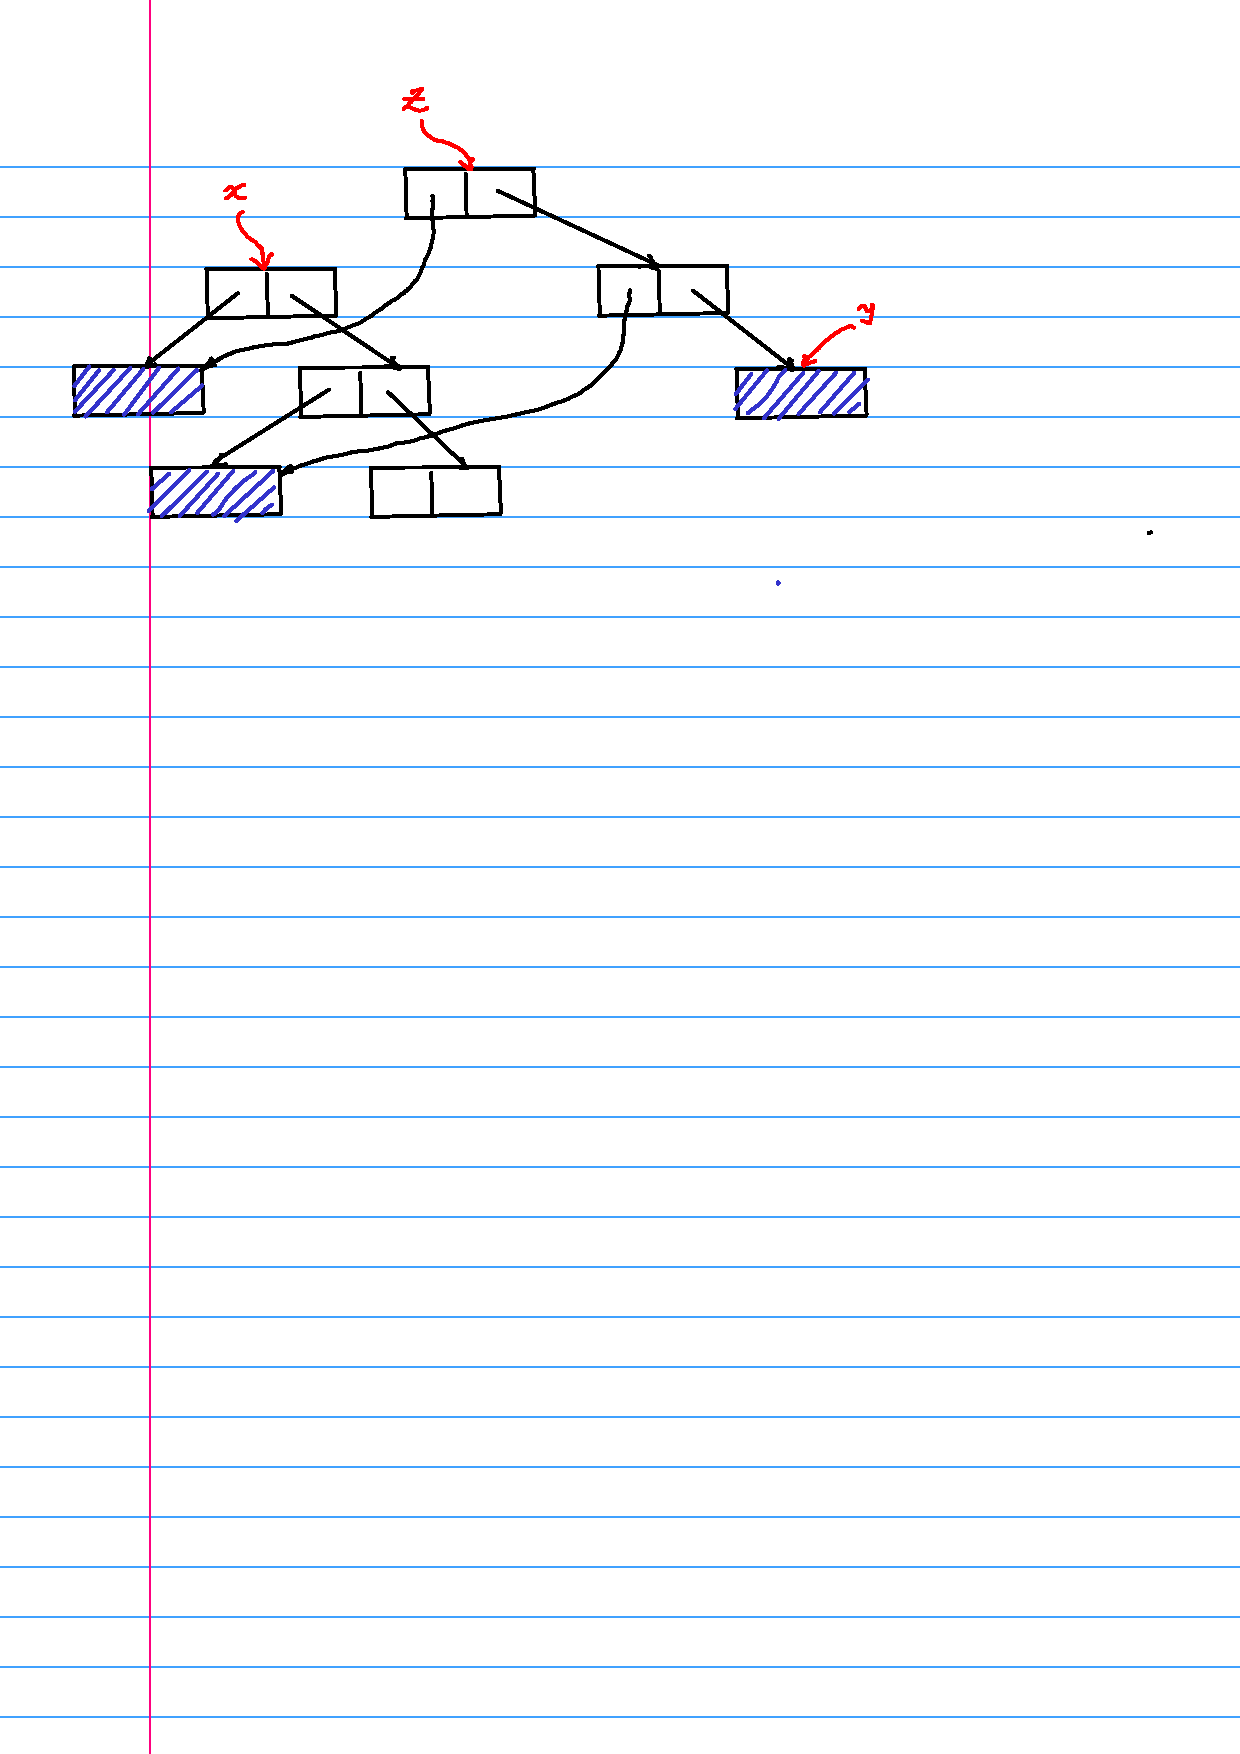
\includegraphics[width=.45\textwidth]{motiv-example}
      %%%%%%%%%%%%%%%%%%%%%Uday's stuff%%%%%%%%%%%%%%%%%%%%%%%%%
\psset{xunit=1mm, yunit=.8mm}
\psset{linewidth=.3mm}
\begin{pspicture}(0,17)(70,57)
%  \psframe(0,17)(70,57)
  %%%%%%%%%%%%%%%%%%%%%%%%%%%%%%%%%%%%%%%%%%%%%%%%%%%%%%%%%%%%%%%%
  \putnode{o}{origin}{13}{40}{\TwoCells{o1}{o2}}
  \putnode{a}{o}{-10}{-15}{\psframebox{5}}
  \ncline[offsetB=-.5,nodesepB=.1]{*->}{o1}{a}
  \putnode{y}{o}{-10}{10}{\psframebox[linestyle=none,framesep=.5]{$\px$}}
  \nccurve[nodesepB=-.2,angleA=330,angleB=120]{->}{y}{o}
  \aput[-2.5](.4){\scalebox{1.2}{\psframebox[framesep=.2,linestyle=none,fillstyle=solid,
	fillcolor=white]{$\times$}}}
  %%%%%%%%%%%%%%%%%%%%%%%%%%%%%%%%%%%%%%%%%%%%%%%%%%%%%%
  \putnode{c}{o}{25}{4}{\TwoCells{c1}{c2}}
  \putnode{d}{c}{10}{-10}{\TwoCellsAD{d1}{d2}}
  \putnode{e}{o}{10}{-15}{\TwoCellsAD{e1}{e2}}
  \putnode{f}{d}{13}{-12}{\TwoCellsAD{f1}{f2}}
  \ncline[nodesepB=-.5]{*->}{c2}{d}
  \ncline[nodesepB=-.5,linewidth=.7]{->}{c2}{d}
  \nccurve[ncurv=1,angleA=235,angleB=45]{*->}{c1}{a}
  \aput[-3.5](.2){\scalebox{1.2}{\psframebox[framesep=.2,linestyle=none,fillstyle=solid,
	fillcolor=white]{$\times$}}}
%  \putnode{g}{e}{-6}{-13}{\TwoCellsAD{g1}{g2}}
  \nccurve[nodesepB=-.5,angleA=240,angleB=30]{*->}{d1}{e}
  \aput[-2.5](.5){\scalebox{1.2}{\psframebox[framesep=.2,linestyle=none,fillstyle=solid,
	fillcolor=white]{$\times$}}}
  \ncline[angleA=300,angleB=110]{*->}{d2}{f}
  \ncline[angleA=300,angleB=110,linewidth=.7]{->}{d2}{f}
  \putnode{w}{c}{-8}{11}{\psframebox[linestyle=none,framesep=.2]{$\pz$}}
  \putnode{ww}{c}{30}{-5}{\psframebox[linestyle=none,framesep=.2]{$\py$}}
  \nccurve[nodesepB=-.2,angleA=330,angleB=120,linewidth=.7]{->}{w}{c}
  %%%%%%%%%%%%%%%%%%%%%%%%%%%%%%%%%%%%%%%%%%%%%%%%%%%%%%%%%%%%%%%%%%
  \ncline[offsetB=-.5,nodesepB=.1]{*->}{o2}{e}
  %\ncline[offsetB=-.1,nodesepB=-.2]{*->}{e1}{g}
  \nccurve[nodesepB=-.3,angleA=270,angleB=90,offsetB=.5]{->}{ww}{f}
  \aput[-3.5](.5){\scalebox{1.2}{\psframebox[framesep=.2,linestyle=none,
        fillstyle=solid, fillcolor=white]{$\times$}}}
  %%%%%%%%%%%%%%%%%%%%%%%%%%%%%%%%%%%%%%%%%%%%%%%%%%%%%%%%%%%%%%%%%%
\end{pspicture}
 \\ \\
      \renewcommand{\arraystretch}{.9}
      \begin{tabular}[t]{p{0.9\columnwidth}}
        (b) Memory graph at $\pi$.  \scalebox{.7}{\TwoCellsAD{a1}{a2}}
        denotes a closure. Thick edges denote live links. Traversal
        stops at edges marked $\times$ during garbage collection for
        a liveness-based collector.
      \end{tabular}
    \end{tabular} 
  \end{pspicture}
%  \vspace*{-3ex}
  \caption{Example Program and its Memory Graph}\label{fig:mot-example}
\end{figure}

